\documentclass[11pt]{article}
\usepackage{times}
\usepackage{amsmath,amsthm,amssymb,mathtools,setspace,enumitem,epsfig,titlesec,verbatim,color,array,multirow,comment,graphicx,hyperref,blkarray}
%\usepackage[sort&compress]{natbib} % ProcB
\usepackage[super,sort&compress,comma]{natbib} % NComms
\usepackage[bf,small]{caption}
\usepackage[export]{adjustbox}
\usepackage[top=2.5cm,left=2.8cm,right=2.8cm,bottom=3.2cm]{geometry} 
\smallskip 

\definecolor{darkred}{rgb}{0.6,0,0}
\definecolor{darkblue}{rgb}{0,0.3,0.8}

\newcommand{\christian}[1]{\textcolor{blue}{{\bf CH:} #1}} 

\titleformat{\section}{\sffamily \fontsize{12}{20}\bfseries}{\thesection}{1em}{}
\titleformat{\subsection}{\sffamily \fontsize{11}{20}\bfseries}{\thesubsection}{1em}{}

\renewcommand{\figurename}{Supplementary Figure}


\newcommand{\FigIllustration}{{\bf Fig.~1}}

\newtheoremstyle{plainCl1}% name
{9pt}%      Space above, empty = 'usual value'
{15pt}%      Space below
{\it}% 	   Body font
{}%         Indent amount (empty = no indent, \parindent = para indent)
{\bfseries}% Thm head font
{.}%        Punctuation after thm head
{2mm}% Space after thm head: \newline = linebreak
{}%         Thm head spec

\newtheoremstyle{plainCl2}% name
{9pt}%      Space above, empty = 'usual value'
{15pt}%      Space below
{\it}% 	   Body font
{}%         Indent amount (empty = no indent, \parindent = para indent)
{\bfseries}% Thm head font
{.}%        Punctuation after thm head
{4mm}% Space after thm head: \newline = linebreak
{}%         Thm head spec

\theoremstyle{plainCl1}
\newtheorem{theorem}{Theorem}
\newtheorem{Prop}{Proposition}
\newtheorem{definition}{Definition}

\theoremstyle{plainCl2}
\newtheorem{lemma}{Lemma}
\newtheorem{proposition}{Proposition}
\newtheorem{Corollary}{Corollary}


\newcommand{\ALLD}{\emph{D}}

\newcommand{\A}{\mathbf{A}}
\newcommand{\abf}{\mathbf{a}}
\newcommand{\T}{\mathbf{T}}
\newcommand{\ubf}{\mathbf{u}}
\newcommand{\C}{\mathrm{C}}
\newcommand{\D}{\mathrm{D}}

\title{\sffamily \Large Supplementary Information\\[0.1cm] {\bfseries Introspection dynamics in asymmetric multiplayers games}}
\date{\empty}
\author{\parbox[c]{16cm}{\centering \onehalfspacing \fontsize{11}{12}\selectfont Marta Couto$^1$ and Saptarshi Pal$^1$\\[0.2cm]
$^1$Max Planck Research Group Dynamics of Social Behavior, Max Planck Institute for Evolutionary Biology, 24306~Ploen, Germany}}


\begin{document}
\maketitle
\onehalfspacing
\section*{Supplementary Figures}
\begin{figure}[h!]
\centering
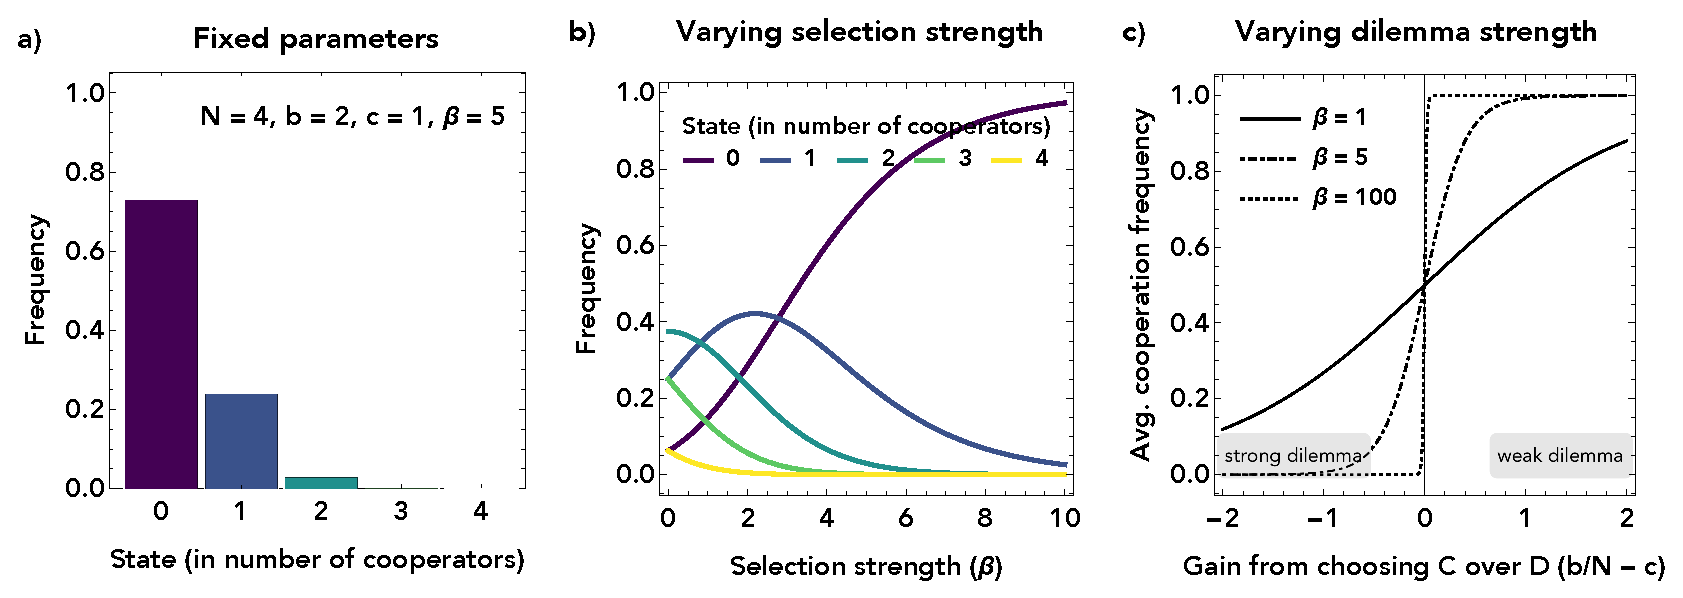
\includegraphics[width =  \textwidth]{figures/figure1.eps}~\\[0.4cm]
\caption{\onehalfspacing
\textbf{Symmetric linear public goods game.}
a) Frequency of each state in the stationary distribution of introspection dynamics. As players are indistinguishable here, each state can be fully defined by the number of cooperators. Parameters: $N = 4$, $b = 2$, $c = 1$ and $\beta = 5$. b) For the same game parameters ($N = 4$, $b = 2$ and $c = 1$), we now show the frequency of each state (same color code as in panel a) for varying selection strength $\beta$. Comparing neutrality ($\beta = 0$) with low to intermediate $\beta$ values, we see that selection favors states other than 0 cooperators. Indeed, up to $\beta \approx 3$, state $0$ is not even the most frequent. c) Average cooperation frequency for varying dilemma strength. We use as a measure of the dilemma strength the marginal gain by choosing to cooperate over choosing to defect, $b/N - c$. When this quantity is low, we say there is a ``strong dilemma”, where there is no individual advantage to cooperate, whereas when the marginal gain is high, we say there is a ``weak dilemma” (or no dilemma), where to cooperate becomes advantageous. Typically, a linear public goods dilemma is defined as having a negative marginal gain (see conditions above). Here, we show the whole parameter range for completeness and a full grasp of this game. We also show the result for different values of selection strength, $\beta = 1, 5$ and $100$. For high $\beta$, we confirm the classical prediction that, assuming a negative marginal gain, defection is dominant. For low $\beta$, however, we see again that some cooperation is possible. }
\label{Fig:LPGG-symmetric}
\end{figure}
\clearpage

\begin{figure}
\centering
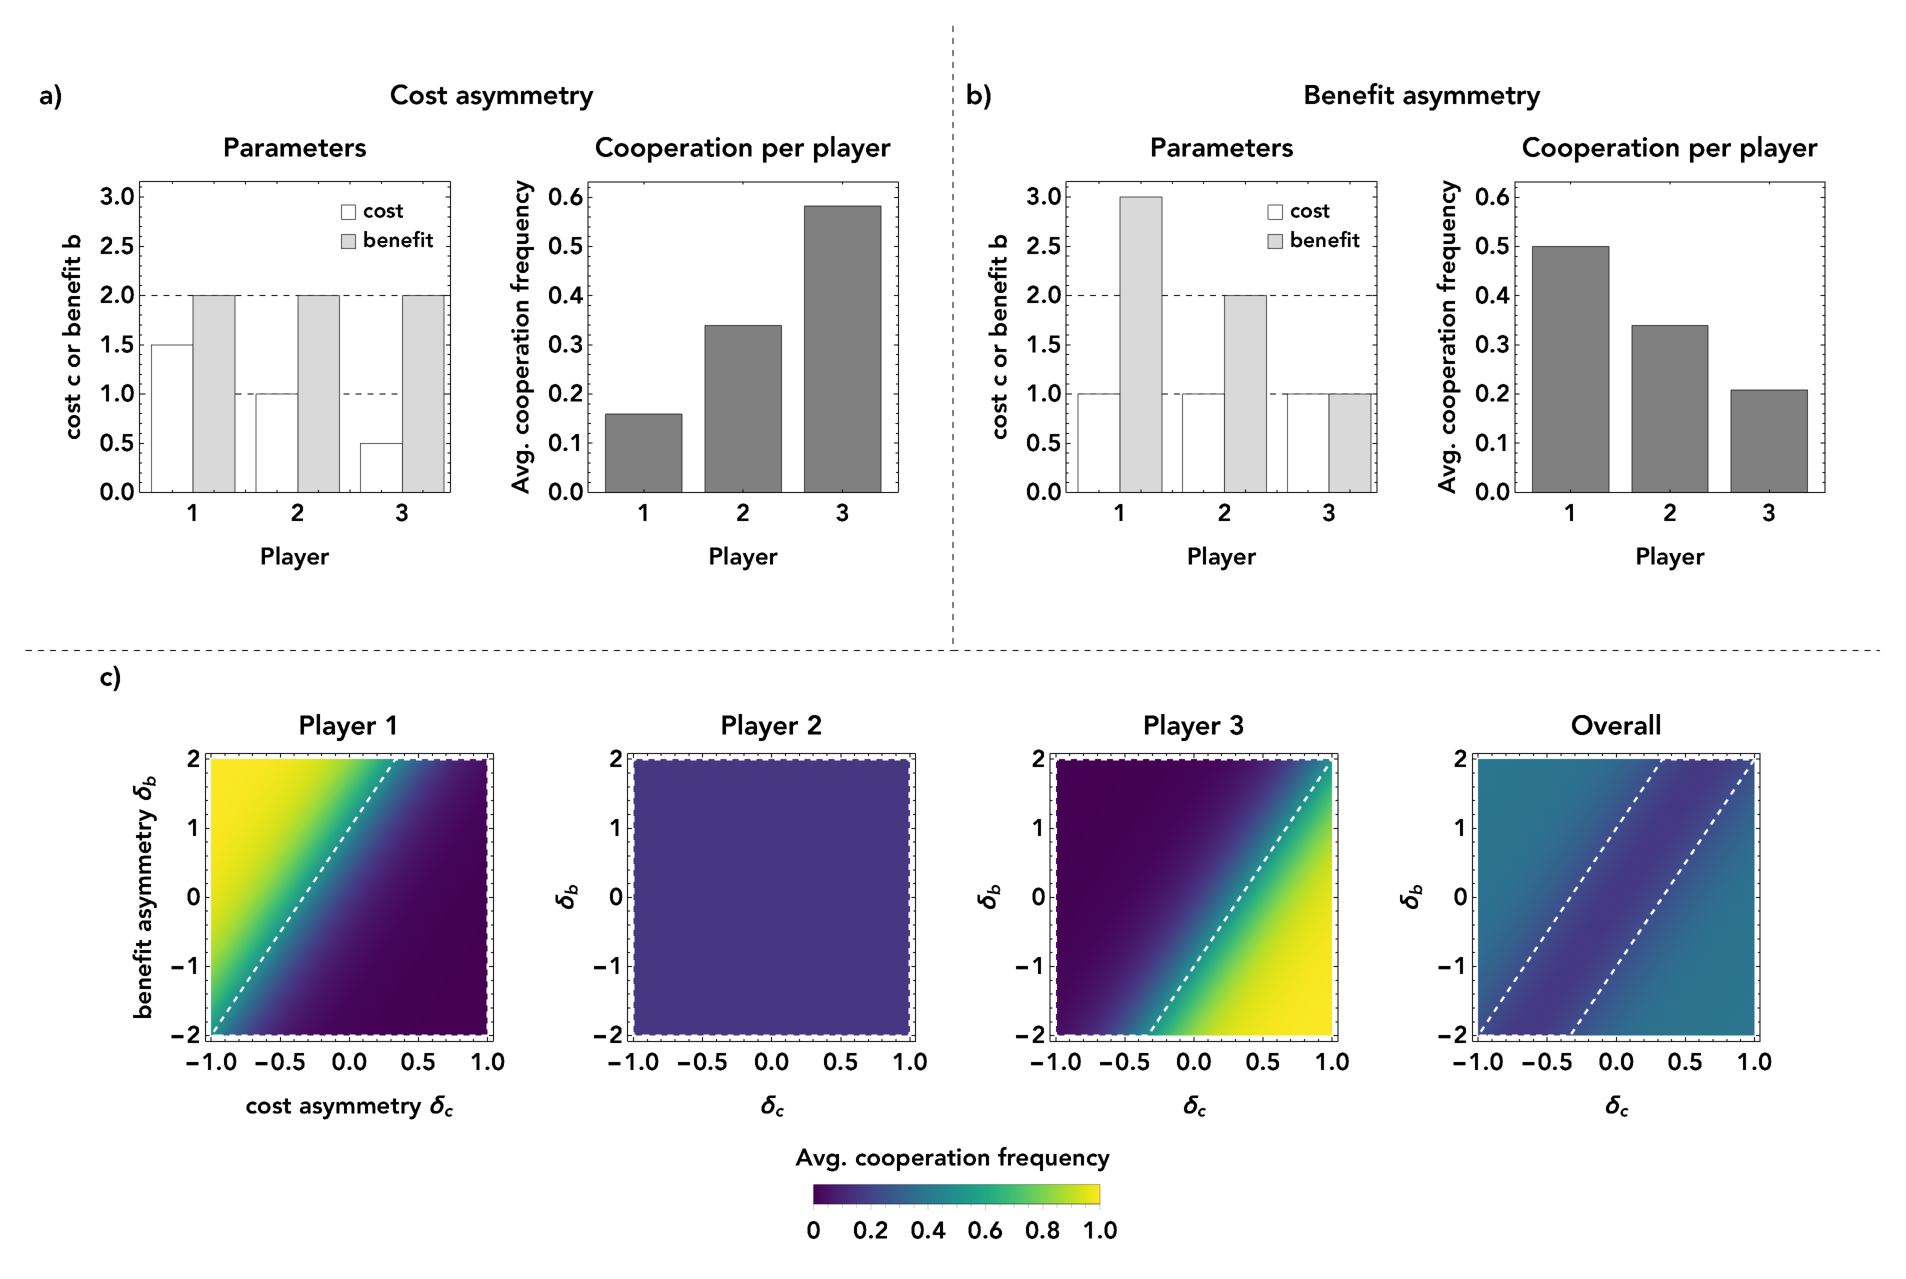
\includegraphics[width =  \textwidth]{figures/figure2.eps}~\\[0.4cm]
\caption{\onehalfspacing
\textbf{Asymmetric linear public goods game.} In the upper panels a) and b), we show the parameter values of the cost and benefit on the left and the average cooperation frequency on the right, of each player. Parameters: $N=3$, $\bar{c} = 1$, $\bar{b} = 2$, $\beta = 2$, where $\bar{c}$ and $\bar{b}$ are the mean values and are represented by black, dashed lines. In a) the cost varies among the 3 players by $\delta_c = 0.5$, such that players have costs of $\bar{c} + \delta_c $, $\bar{c}$, and $\bar{c} - \delta_c$ (in this case, $1.5$, $1$, and $0.5$), while the benefit is the same. Conversely, in b) the benefit varies among the 3 players, by $\delta_b = 1$, such that players have benefits of $\bar{b} + \delta_b $, $\bar{b}$, and $\bar{b} - \delta_b$ (in this case, $3$, $2$, and $1$), while the cost is the same. In c), we vary the asymmetry strengths $\delta_c $ and $\delta_b$ at the same time and show both each player’s average cooperation frequency and the overall average cooperation frequency. The area within the white dashed lines represents the parameter range for which the marginal gain by cooperating is negative, for each single player and, in the right-most panel, for all players. Parameters: $N=3$, $\bar{c} = 1$, $\bar{b} = 2$, $\beta = 5$.
}
\label{Fig:LPGG-asymmetric}
\end{figure}
\end{document}